\appendix

% Reset section format for appendix (no РОЗДІЛ prefix)
\titleformat{\section}
  {\centering\bfseries\Large}
  {\thesection.}
  {0.5em}
  {}

% Reset ToC section format for appendix
\addtocontents{toc}{\protect\renewcommand*{\protect\cftsecpresnum}{}}
\addtocontents{toc}{\protect\setlength{\protect\cftsecnumwidth}{1.5em}}

\addcontentsline{toc}{section}{ДОДАТКИ}

% Visible ДОДАТКИ heading
\begin{center}
{\bfseries\Large ДОДАТКИ}
\end{center}
\vspace{1cm}

%% Додаток А — Обов'язковий додаток (§13 Наказу МОН №40)
\section{Список публікацій Д. С. Шепілева за темою дисертації та відомості про апробацію результатів дисертації}\label{app:publications}

\printpratsi

\setlength \tabcolsep {3pt}

\begin{center}
\begin{spacing}{1}

\begin{longtable}{|p{0.6\linewidth}|p{0.35\linewidth}|}
  \caption{Відомості про апробацію результатів дисертації}
  \label{tab:approbation} \\

\hline
\hfil \textbf{Назва заходу} &

\hfil \begin{tabular}{c}
     \textbf{Місце та дата}  \\
     \textbf{проведення}
\end{tabular}

\\

\hline

\endfirsthead

\multicolumn{2}{r}%
{{\itshape Продовження таблиці \thetable{} }} \\
\hline

\hfil \textbf{Назва заходу} &

\hfil \begin{tabular}{c}
     \textbf{Місце та дата}  \\
     \textbf{проведення}
\end{tabular}

\\

\hline

\endhead

\endfoot

\endlastfoot

3rd International Workshop on Augmented Reality in Education (AREdu 2020) & Кривий Ріг, 13 травня 2020~р. \\\hline

XII International Conference on Mathematics, Science and Technology Education (ICon-MaSTEd 2020) & Кривий Ріг, 15--17 жовтня 2020~р. \\\hline

International Workshop on Computer Science \& Software Engineering at Schools and in the Workplace (CS\&SE@SW 2020) & Кривий Ріг, 27 листопада 2020~р. \\\hline

9th Workshop on Cloud Technologies in Education (CTE 2021) & Кривий Ріг, 17 грудня 2021~р. \\\hline

Digital Humanities Workshop (DHW 2021) & Київ, 23 грудня 2021~р. \\\hline

Міжнародна науково-практична конференція <<Наука, освіта та суспільство в XXI столітті: наукові ідеї та механізми реалізації>>
 & Кропивницький,
 19 листопада 2022 р. \\\hline

Друга Всеукраїнська науково-практична конференція <<Освіта і наука в умовах інноваційного розвитку суспільства>> &  Дніпро, 25 жовтня 2023 р.\\\hline

11th Illia O. Teplytskyi Workshop on Computer Simulation in Education (CoSinE 2024) & Кривий Ріг, 15 травня 2024~р. \\\hline

Міжнародна науково-практична конференція <<Наукова діяльність як шлях формування професійних компетентностей майбутнього фахівця>> & Суми,  5-6 грудня 2024 р.\\\hline

Друга регіональна науково-практична конференція молодих науковців <<Актуальні питання розвитку освіти та управління освітніми закладами>> & Херсон, 30 січня 2025 р. \\\hline

ІІ всеукраїнська науково-практична конференція з міжнародною
участю <<Особистість та освіта в умовах сучасних соціокультурних викликів:
ціннісно-світоглядні та науково-методичні аспекти>>
& Дніпро, 28 лютого 2025 р.\\\hline

III Міжнародна науково-практична
конференція <<Тенденції забезпечення якості освіти>>  &  Дніпро, 11 серпня 2025 р.\\\hline

Міжнародна науково-практична конференція <<Інноваційні тенденції в науці, освіті та технологіях: виклики та перспективи>> & Полтава,
 23 серпня 2025 р.\\\hline

V Міжнародна  наукова конференція <<Інтелектуальний ресурс сьогодення: наукові задачі, розвиток та  запитання>> &  Чернівці, 29 серпня 2025 р.\\\hline

Третя Всеукраїнська науково-практична конференція <<Освіта і наука в умовах інноваційного розвитку суспільства>> &  Дніпро, 30 жовтня 2025 р.\\\hline

Науково-практична конференція «Дев’яті Фльорівські
читання» & Чернігів, 14 листопада 2025 р. \\\hline

Міжнародна науково-технічна інтернет-конференція <<Автоматизація та біомедичні і комп’ютерні технології>>
 & Дніпро, 13 березня
 2026 р. \\\hline

\end{longtable}

\end{spacing}
\end{center}


%%% Додаток Б
\section{Довідки про впровадження результатів дослідження}\label{app:textbook}

\begin{enumerate}[label=\arabic*.]
	\item Комунальний заклад вищої освіти <<Дніпровська академія неперервної освіти>> Дніпропетровської обласної ради>>
	\item Національний університет <<Чернігівський колегіум>> імені Т. Г. Шевченка
\end{enumerate}

\clearpage

\noindent 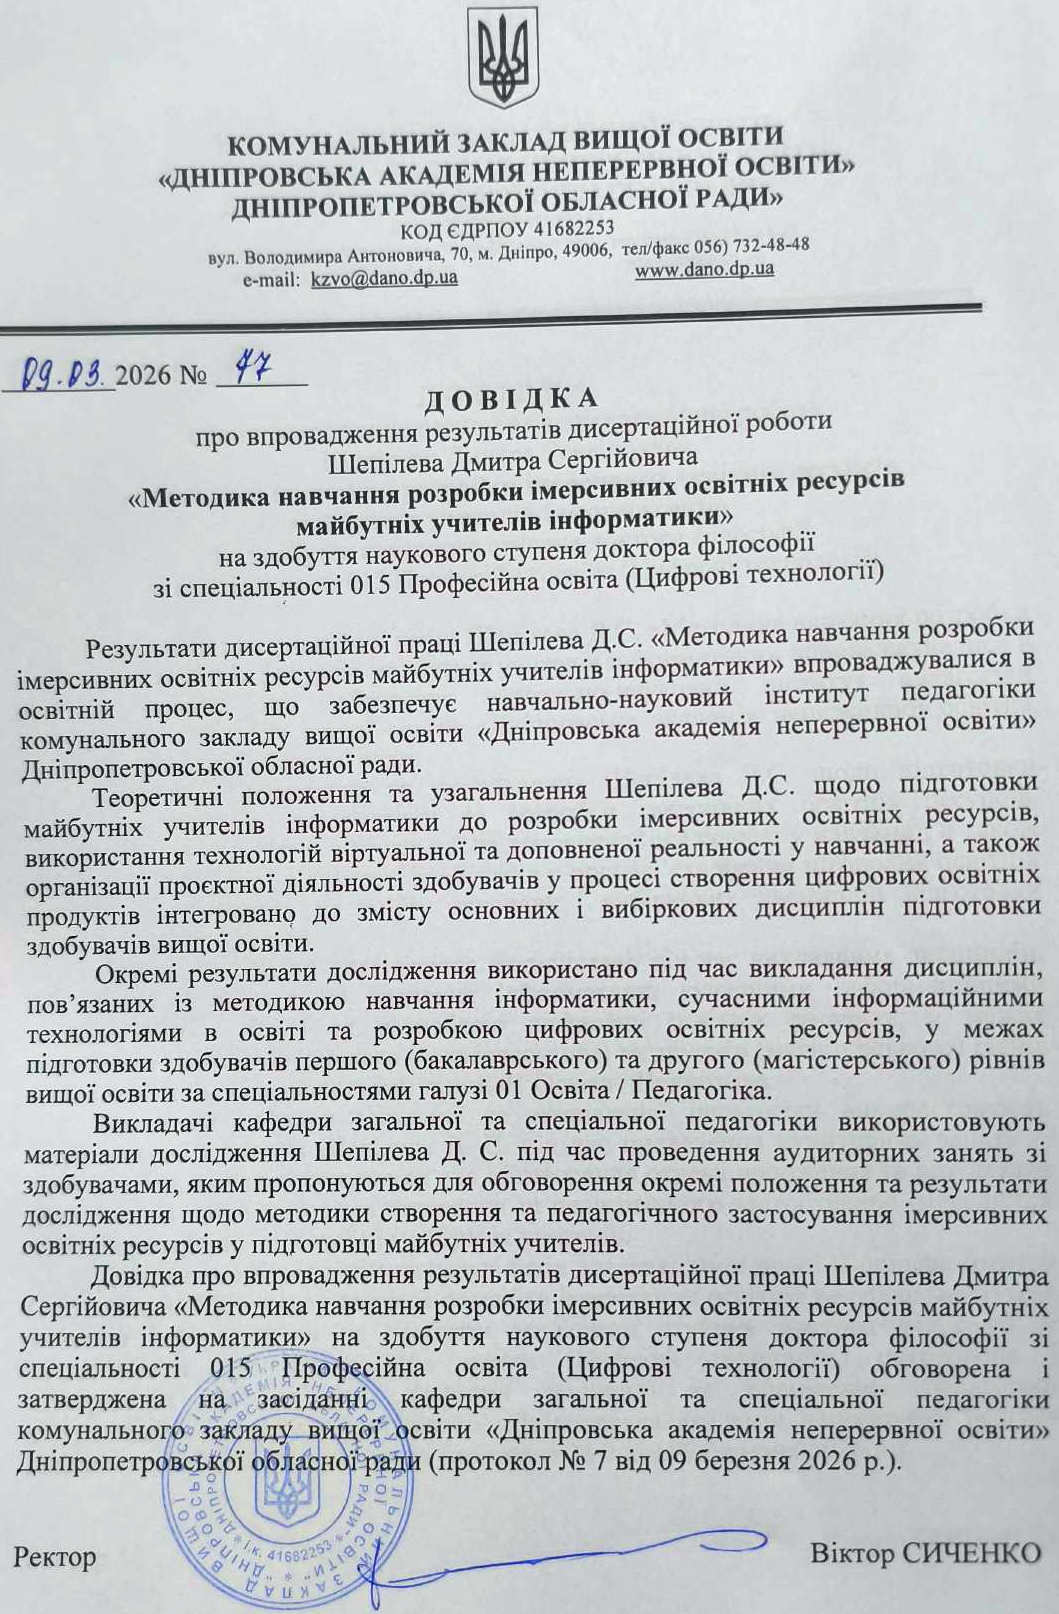
\includegraphics[width=\linewidth]{figures/dovidka_1}

\noindent 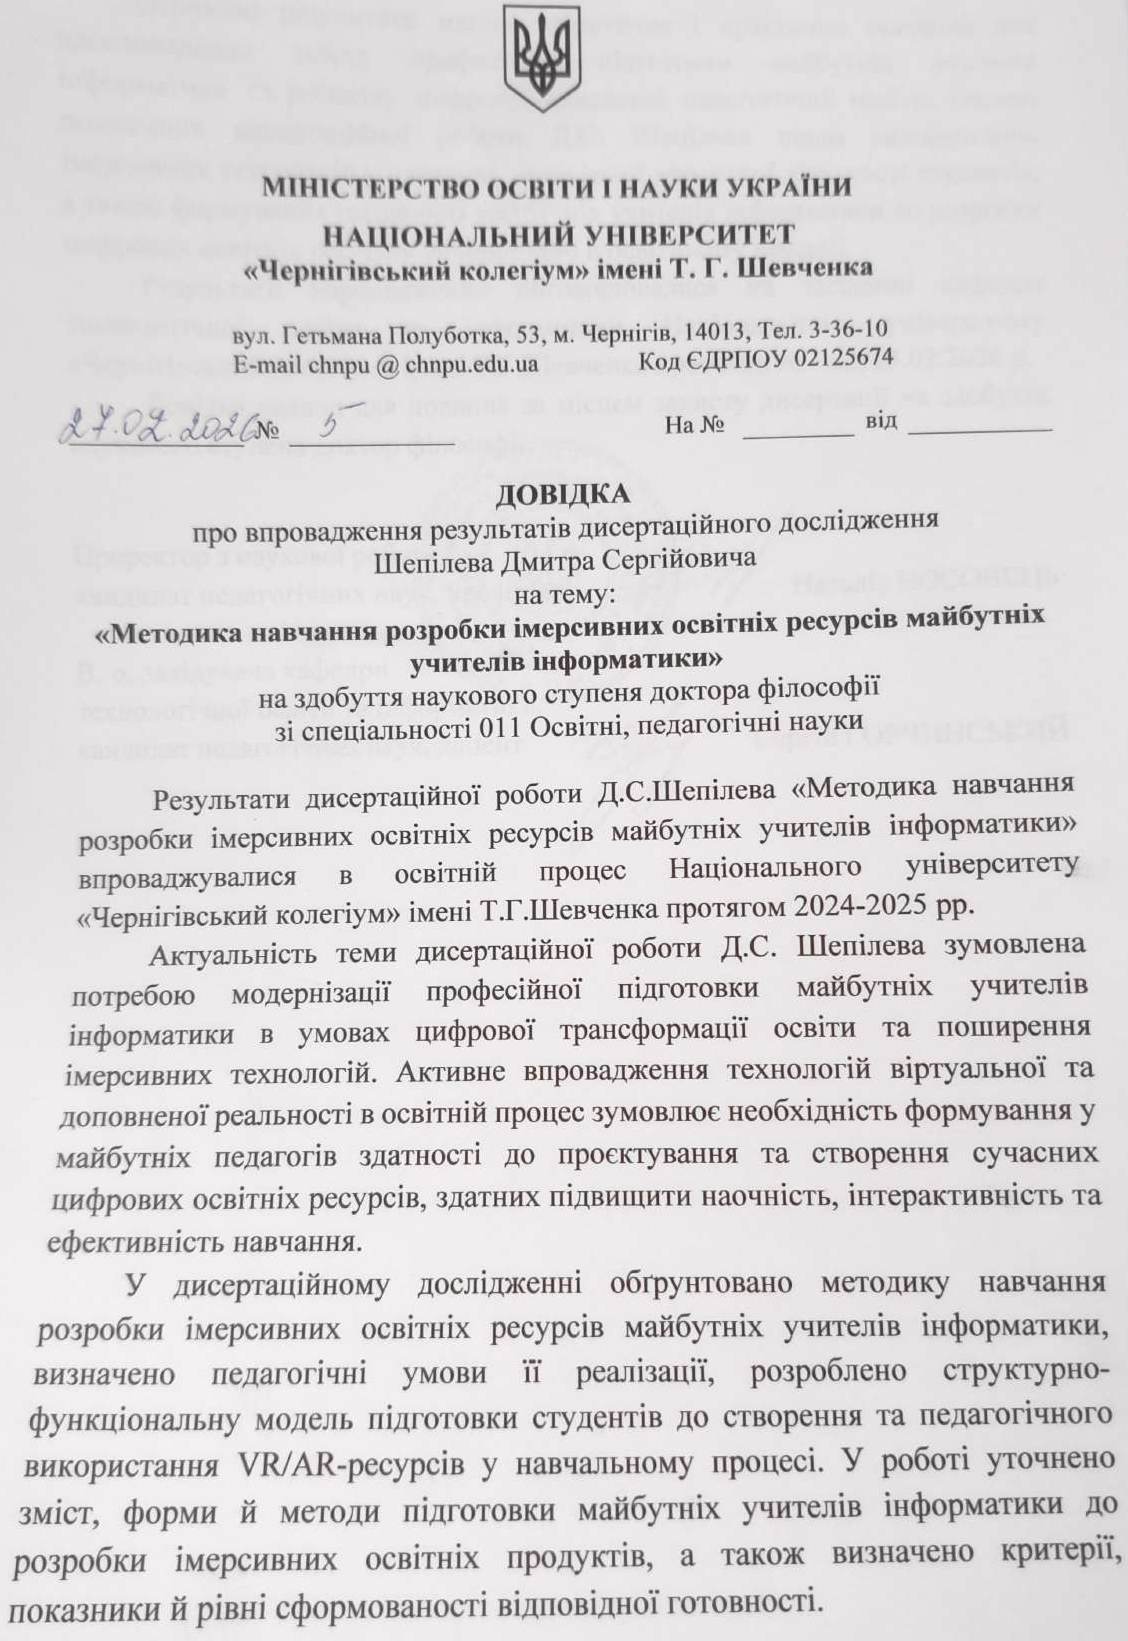
\includegraphics[width=\linewidth]{figures/dovidka_2_1}

\noindent 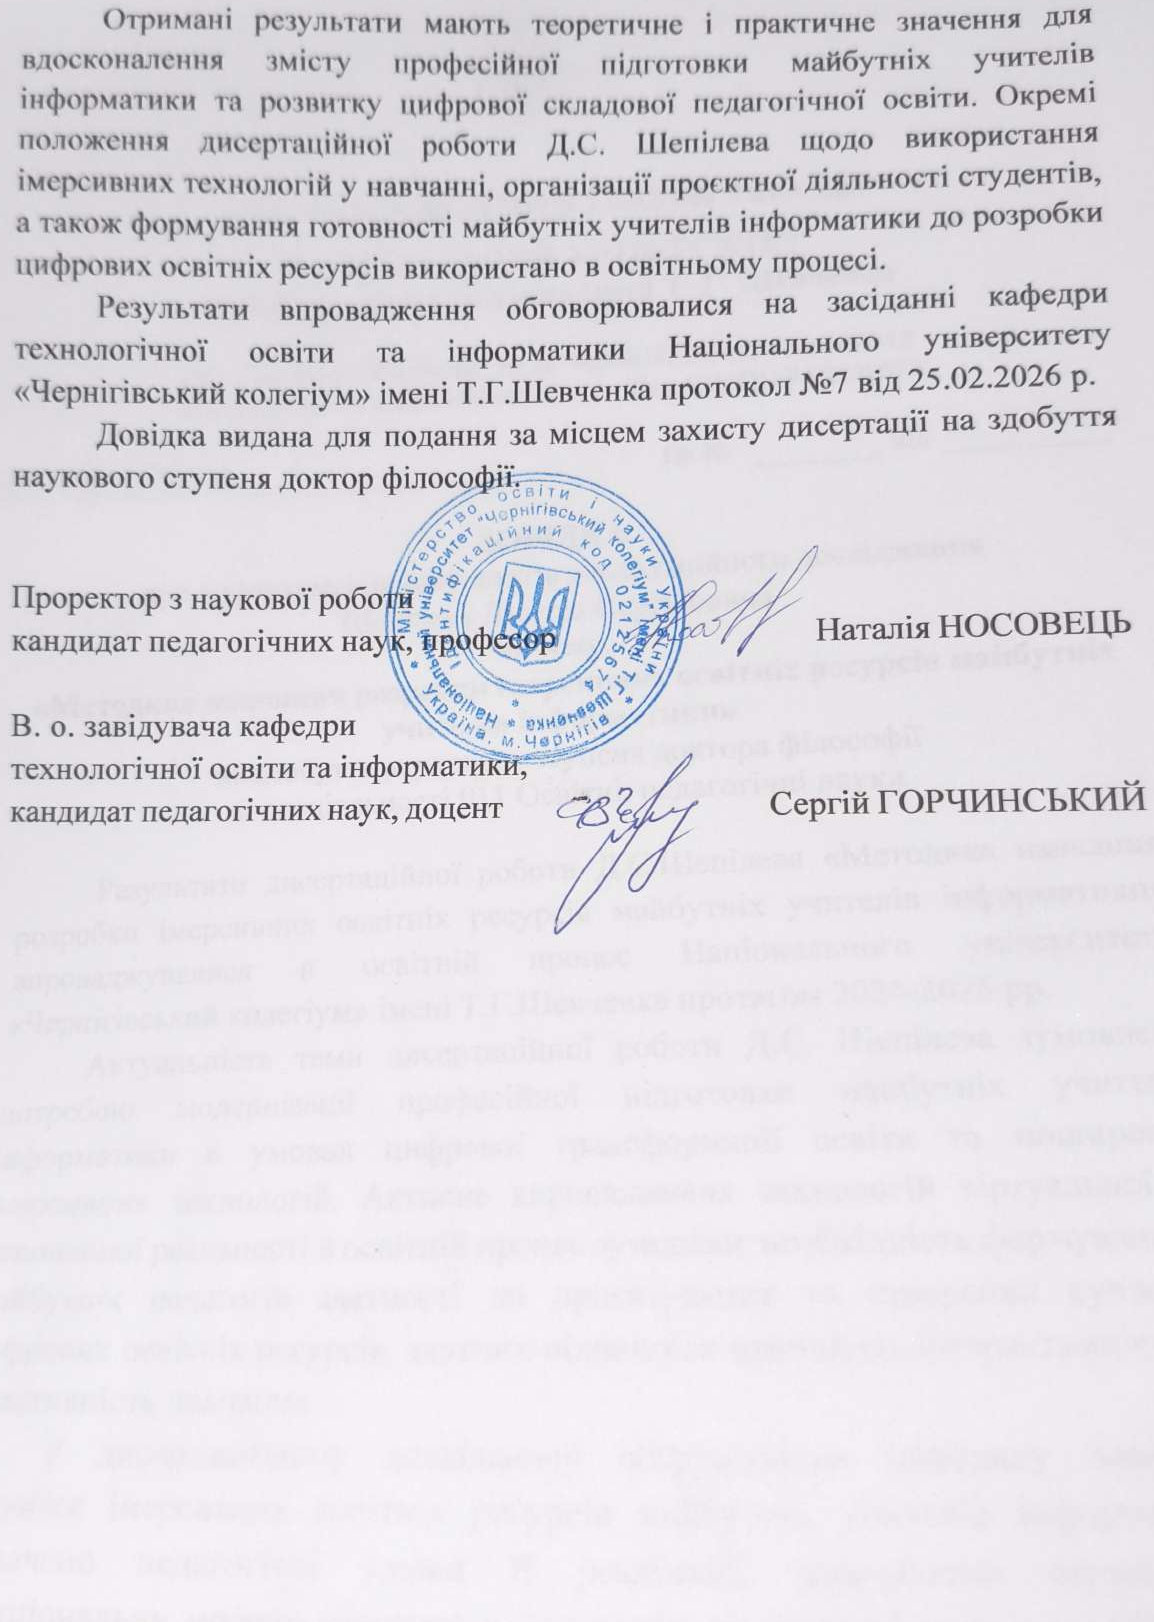
\includegraphics[width=\linewidth]{figures/dovidka_2_2}

%%% Додаток Б
%\section{Навчальний посібник з WebAR}\label{app:textbook}
%
%Навчальний посібник <<Розробка WebAR-застосунків для освіти>> структуровано у 10 розділів, що послідовно охоплюють всі аспекти створення освітніх застосунків з доповненою реальністю у браузері:
%
%\begin{enumerate}
%    \item Вступ до WebAR
%    \item Інструменти розробки (JavaScript, локальні сервери, ngrok, віддалене налагодження)
%    \item Як AR працює у браузерах (WebGL, Three.js, накладання камери)
%    \item Відстеження зображень (MindAR NFT, маркери, 3D-моделі, GLTF/GLB)
%    \item Відстеження обличчя (орієнтири, окклюдери, маски, перемикання камери)
%    \item Відстеження простору (WebXR Device API, hit testing, розміщення на поверхнях)
%    \item Інтеграція машинного навчання (TensorFlow.js, handpose, face-api.js)
%    \item Інші технології WebAR (A-Frame, model-viewer, 8th Wall, Zappar)
%    \item Висновки
%    \item Лабораторний практикум (10 варіантів творчих завдань)
%\end{enumerate}
%
%Повний текст посібника подано в електронному додатку.
%
%%% Додаток В
%\section{Лабораторний практикум}\label{app:labs}
%
%Лабораторний практикум складається з 10 варіантів творчих завдань з 3D-моделювання та доповненої реальності. Кожний варіант включає:
%\begin{itemize}
%    \item завдання на створення 3D-моделей у форматі GLTF/GLB;
%    \item завдання на розробку WebAR-застосунку з відстеженням зображень;
%    \item завдання на розробку WebAR-застосунку з відстеженням обличчя;
%    \item творче завдання на інтеграцію моделей машинного навчання у WebAR.
%\end{itemize}
%
%%% Додаток Г
%\section{Структура курсу <<Синтетична реальність в освіті>> у LMS Moodle}\label{app:moodle}
%
%Курс розгорнуто на платформі moodle.kdpu.edu.ua і структуровано у 18 тижневих модулів (лютий~-- червень 2025):
%
%\begin{longtable}{|p{0.14\textwidth}|p{0.79\textwidth}|}
%\hline
%Тиждень 1 & Вступ. Реєстрація, знайомство з курсом \\
%\hline
%Тиждень 2 & Вступ до WebAR \\
%\hline
%Тиждень 3 & Інструменти розробки WebAR \\
%\hline
%Тиждень 4 & Як AR працює у браузерах \\
%\hline
%Тиждень 5 & Three.js: основи 3D-графіки \\
%\hline
%Тиждень 6 & Відстеження зображень (Image Tracking) \\
%\hline
%Тиждень 7 & Відстеження зображень: практикум \\
%\hline
%Тиждень 8 & Відстеження обличчя (Face Tracking) \\
%\hline
%Тиждень 9 & Відстеження обличчя: практикум \\
%\hline
%Тиждень 10 & Відстеження простору (World Tracking) \\
%\hline
%Тиждень 11 & WebXR Device API \\
%\hline
%Тиждень 12 & Інтеграція машинного навчання \\
%\hline
%Тиждень 13 & TensorFlow.js та Teachable Machine \\
%\hline
%Тиждень 14 & Інші технології WebAR \\
%\hline
%Тиждень 15 & A-Frame та model-viewer \\
%\hline
%Тиждень 16 & Віртуальна хімічна лабораторія \\
%\hline
%Тиждень 17 & Підсумковий проєкт \\
%\hline
%Тиждень 18 & Захист проєктів та рефлексія \\
%\hline
%\end{longtable}
%
%%% Додаток Д
%\section{Віртуальна хімічна лабораторія}\label{app:anchem}
%
%Віртуальну хімічну лабораторію з доповненою реальністю (anchem-ar) розроблено як практичний приклад освітнього WebAR-застосунку для якісного аналізу хімічних речовин. Застосунок демонструє інтеграцію технологій MindAR та Three.js для створення інтерактивного навчального середовища.

\label{last_page}
